\documentclass{article}

\usepackage{ctex,amsmath,graphicx}
\title{电流电离室}
\date{}

\begin{document}
    \maketitle
    \section{实验目的}
    \begin{enumerate}
        \item 了解电流电离室的基本原理和特性
        \item 了解微电流测量的基本原理
        \item 学习用电流电离室进行电离辐射测量的基本方法
    \end{enumerate}
    \section{实验原理}
    见预习报告
    \section{实验内容}
    \begin{enumerate}
        \item 测量不同辐照强度下的V-I曲线
        \item 测量不同气压下的V-I曲线
        \item 测量电流电离室轴向分布曲线
        \item 测量不同距离时的照射量率
    \end{enumerate}
    \section{实验数据}
    \subsection{不同辐照强度下的V-I曲线}
    \begin{figure}[htbp]
        \centering
        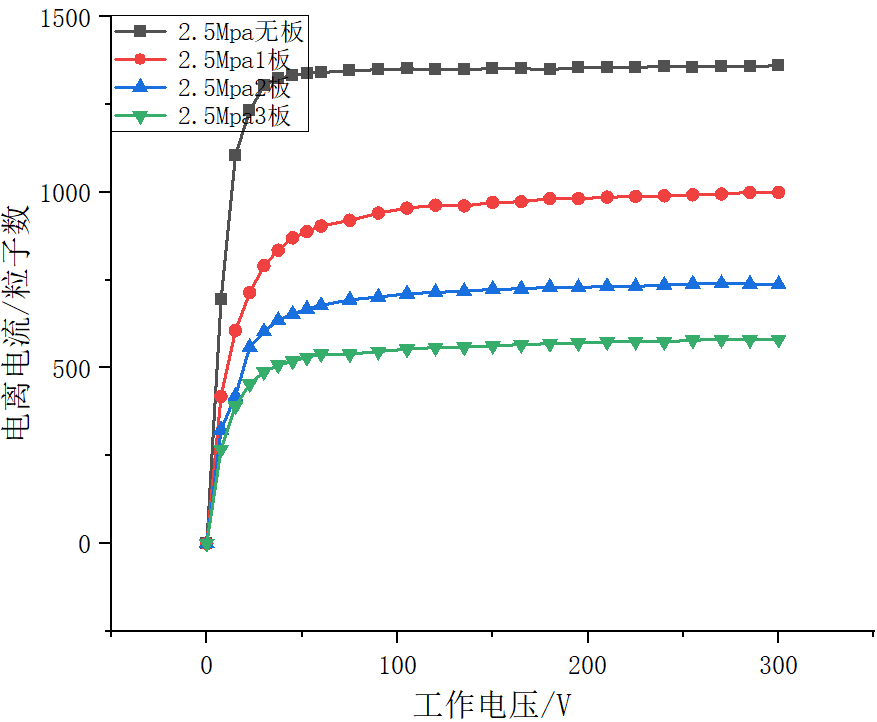
\includegraphics[scale=0.5]{img/2.png}
        \caption{用加的金属板块数的不同来改变辐照强度}
    \end{figure}
    \subsection{测量不同气压下的V-I曲线}
    \begin{figure}[htbp]
        \centering
        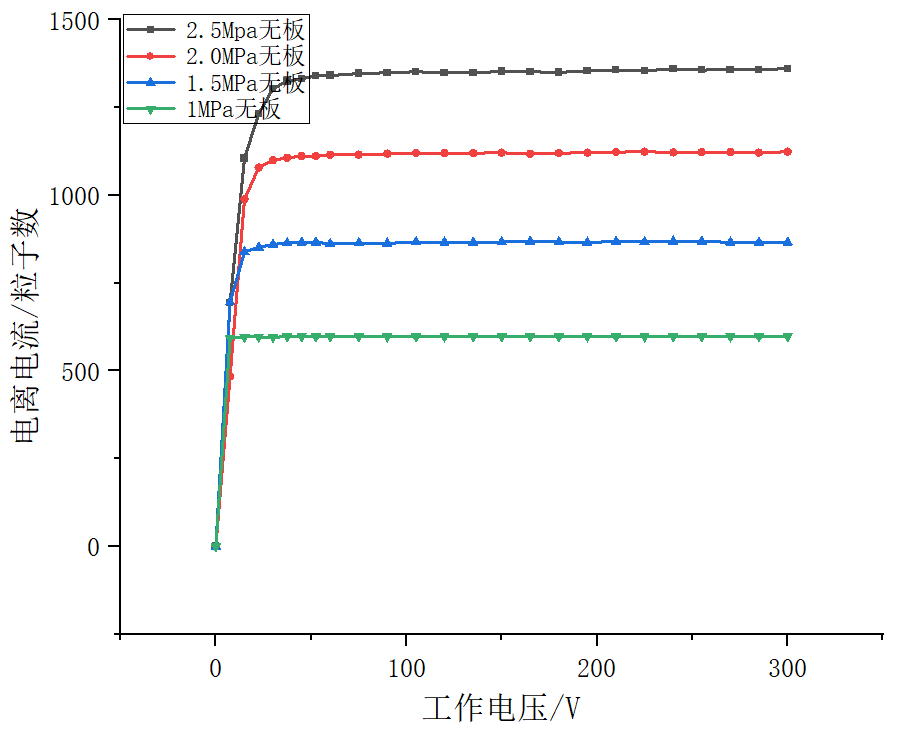
\includegraphics[scale=0.5]{img/1.png}
        \caption{不同气压下的V-I曲线}
    \end{figure}

    \subsection{测量电离电流的轴向均匀性}
    \begin{figure}[htbp]
        \centering
        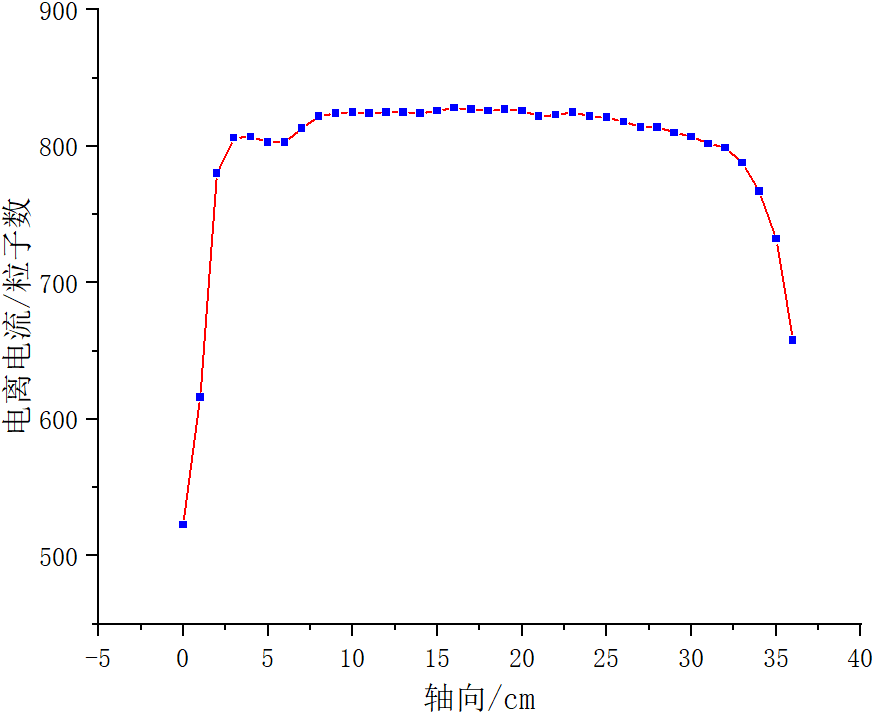
\includegraphics[scale=0.5]{img/3.png}
        \caption{轴向均匀性检验}
    \end{figure}
    \section{思考题}
    \begin{enumerate}
        \item 不能,$\beta$粒子和$\gamma$射线会相互影响,发生核反应
        \item $nEe/ \epsilon$
        \item $\alpha$源的电离电流较大
    \end{enumerate}
\end{document}